 Deep Learning is part of machine learning methods based on artificial neural networks with representation learning. Learning can be supervised, semi-supervised or unsupervised. Part of the theoretical basis underlying Deep Learning  initially emerged as models for understanding learning, that is, how the brain works. Thus, these theories are related with the Neural Networks, one of the areas of Deep Learning  that has grown the most in recent years \cite{goodfellow2016}.

The deep learning area has achieved excellent performance in applications, mainly due to the development of the area and the increase in computational power and the amount of available data \cite{geron2019}. 

Computer vision is another field of Artificial Intelligence (IA), as it also seeks to reproduce some of the human capabilities from autonomous systems. The main interest of computer vision is to make computers perform functions similar to human vision, being able to receive visual data and with them perform recognition, classification and analysis. It is identified that the improvement in the performance of computer vision is strongly linked with the evolution of machine learning.

The old computer vision techniques were almost entirely pipelined by hand, where the features to be extracted and the algorithms used were done manually. This made such techniques more difficult to adapt to different tasks. With the emergence of deep learning, it became possible to use these networks to perform this feature extraction work, in addition to the algorithm part, where machine learn performs the task.

\begin{figure}
    \centering
    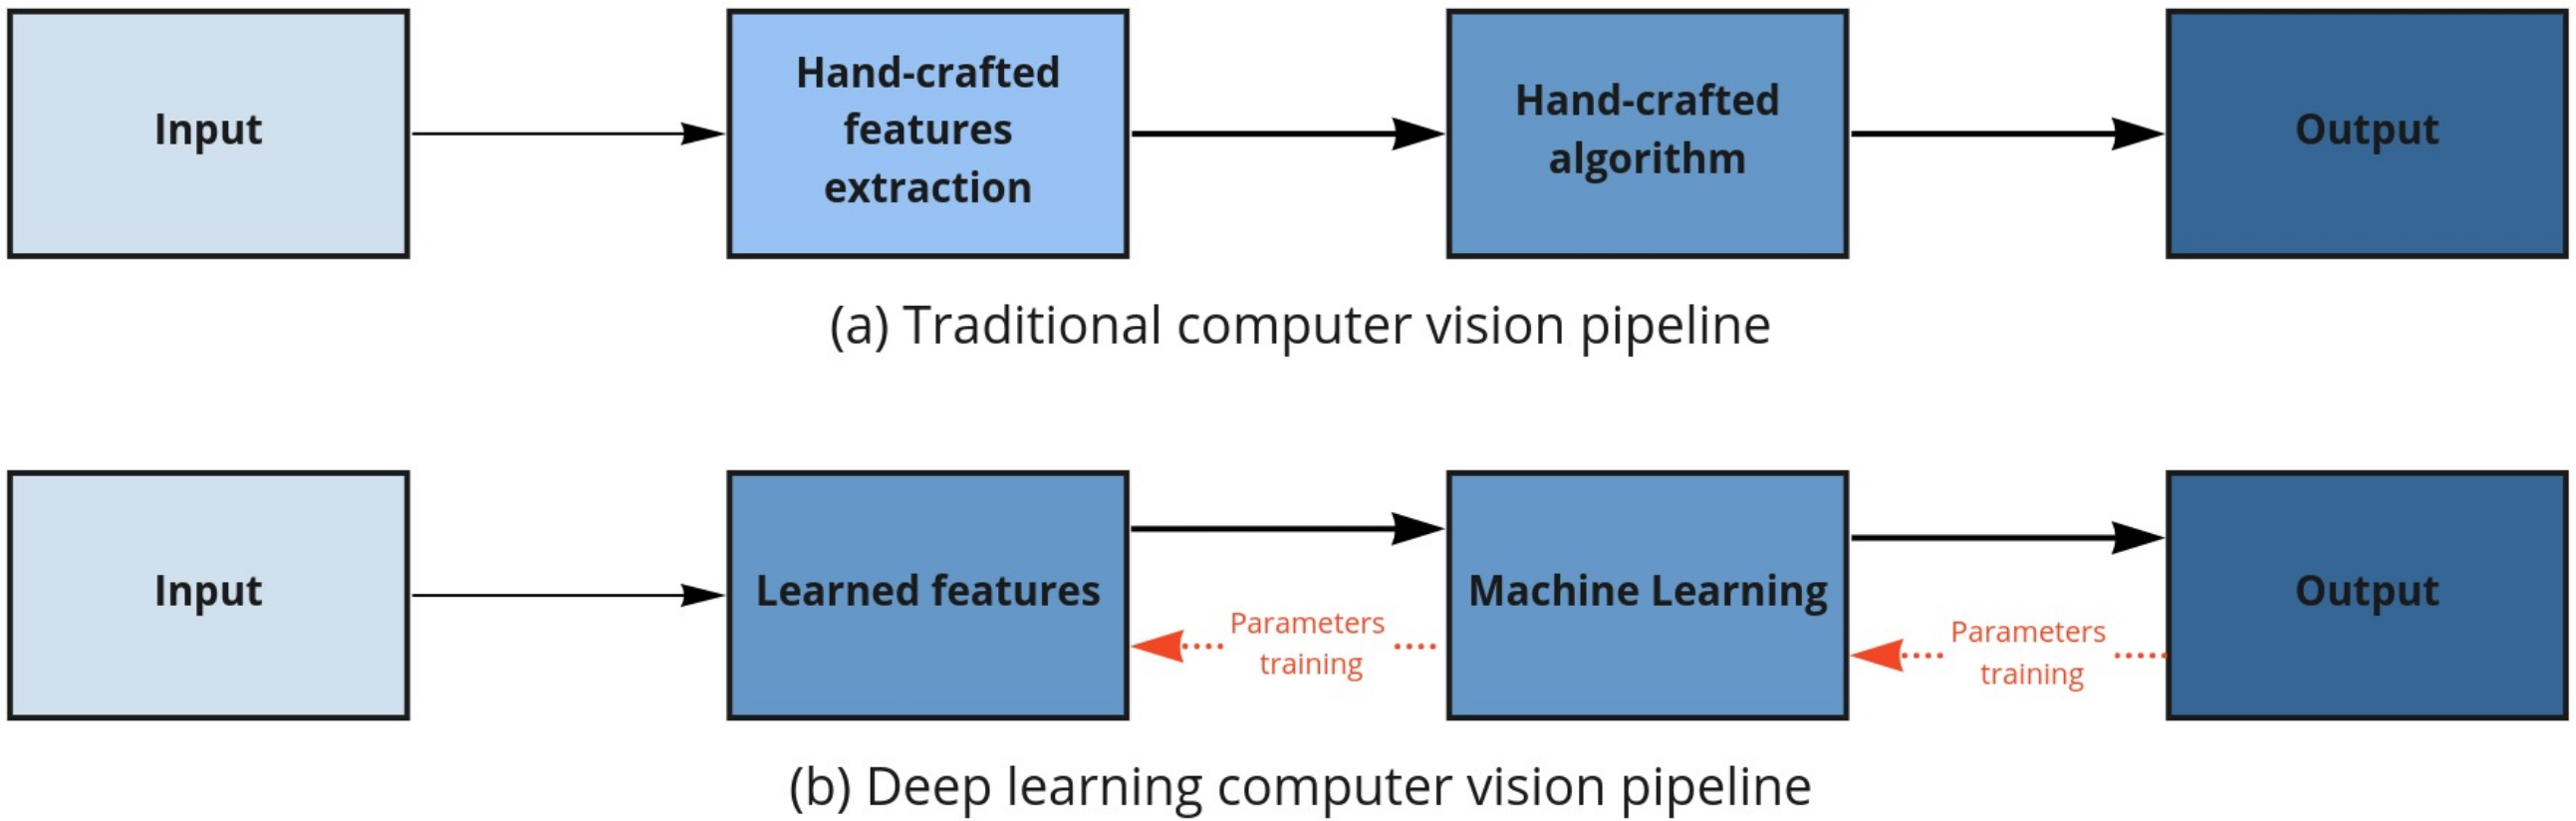
\includegraphics[scale=0.20]{images/cvpipeline.png}
    \caption{Traditional(a) and Deep learnign(b) computer vision pipelines. Inspired in \cite{szeliski2010computer}(Figure 5.2)}
    \label{fig:figurecvpipeline}
\end{figure}

In Figure \ref{fig:figurecvpipeline} we have the representation of the two types of pipeline previously mentioned. The tradicional(\ref{fig:figurecvpipeline} (a)), where the two principal steps, the selection of features to be extract and the algorithm that use these features, are hand-crafted. The Deep learning pipeline(\ref{fig:figurecvpipeline} (b)), where the model learns which features to extract and how use these features to get the desired output. The red arrow in Deep Learning pipeline shows how this type of model use information about the output to adjust the parameters of the network, and consequently, learns.

Among the many deep learning architectures, the Convolutional Neural Networks (CNN) is the most widely used as it is very similar to conventional NN.

\section{Convolutional Neural Networks (CNN)}

In common neural networks we basically use neurons and connections between them to build a model. Convolutional neural networks, on the other hand, have some more structures, which are the reason for their efficiency in working with images. We will see them next.


\subsection{Convolution Operation}

The operation that names the network, the convolution, is an operation performed between two functions. In our case, as we are working with images, we will use discrete convolution.
An important point to note is that mathematically what we will call a convolution is actually a correlation, and the two are almost identical, except for the fact that in the convolution we rotate the filter (kernel) by 180\textdegree . The only advantage we gain from turning the filter before the operation is that we gain the commutative property, which is mathematically useful for proof derivation but not important in Deep Learning  implementation \cite{goodfellow2016}.

In Deep Learning  literature and libraries, including CNN's, it has become common to call the two operations convolution \cite{goodfellow2016}, so we will also use this convention, using convolution without rotating the filter, so a correlation.
The discrete correlation formula is given by:

\begin{equation}
g(x,y)=w(x,y)\star f(x,y)=\sum_{s=-a}^a\sum_{t=-b}^bw(s,t)f(x+s,y+t)
\end{equation}

Where $\star$ represents the correlation operation; $w$ is our filter (kernel), a matrix of numbers, usually with odd square size (to facilitate operations), and $f$, our image, also an matrix. And related to it we have the formula of convolution ($g$):

\begin{equation}
g(x,y)=w(x,y)\ast f(x,y)=\sum_{s=-a}^a\sum_{t=-b}^bw(s,t)f(x-s,y-t)
\end{equation}

As we can see by looking at the two equations, these operations are very simple, being basically a sum of products. In Figure \ref{fig:figure117}, we have a representation of a correlation step, where we can observe the following operation:

%corrigir orientação
\begin{equation}
\begin{split}
w*f(0,0)=\sum_{s=1}^{2}\sum_{t=1}^{2}w(s,t){f}(0-s,0-t)= \\
w(0,0)f(0,0)+w(0,1)f(0,1)+w(0,2)f(0,2) \\
+w(1,0)f(1,0)+w(1,1)f(1,1)+w(1,2)f(1,2) \\
+w(2,0)f(2,0)+w(2,1)f(2,1)+w(2,2)f(2,2)\\
=(-1)\cdot5+(-2)\cdot7+(-1)\cdot0\\
+0\cdot6+0\cdot0+0\cdot1\\
+1\cdot6+2\cdot2+1\cdot2
=-19-0+12=-7
\end{split}
\end{equation}

\begin{figure}
    \centering
    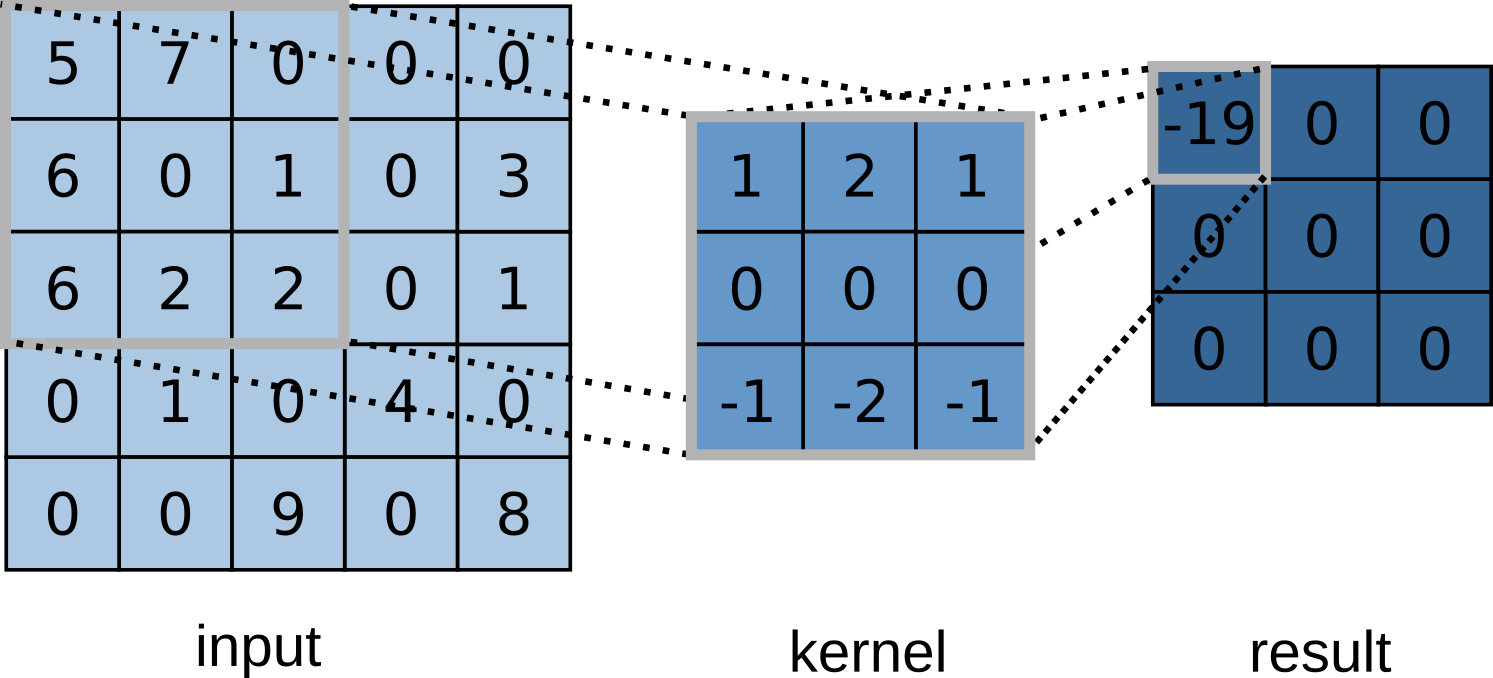
\includegraphics[scale=0.40]{images/figure117.png}
    \caption{Convolution of a 5x5 sized image with a 3x3 sized kernel and its result.}
    \label{fig:figure117}
\end{figure}

The previous example, Figure \ref{fig:figure117}, was quite simple, but we know that in many applications we won't have the input image represented by just a matrix (configuring a grayscale image) but most of the time we will be using images that contain three dimensions. In this case, we will have an image in the RGB model, where three matrices will be present, each one representing a color channel. In Figure \ref{fig:figure118}, there is an example of convolution in RGB images. We can see that now our kernel is also made up of three matrices. An important thing to note is that the number of layers in the filter has to equal the number of channels in the image for the convolution operation to be done.

\begin{figure}
    \centering
    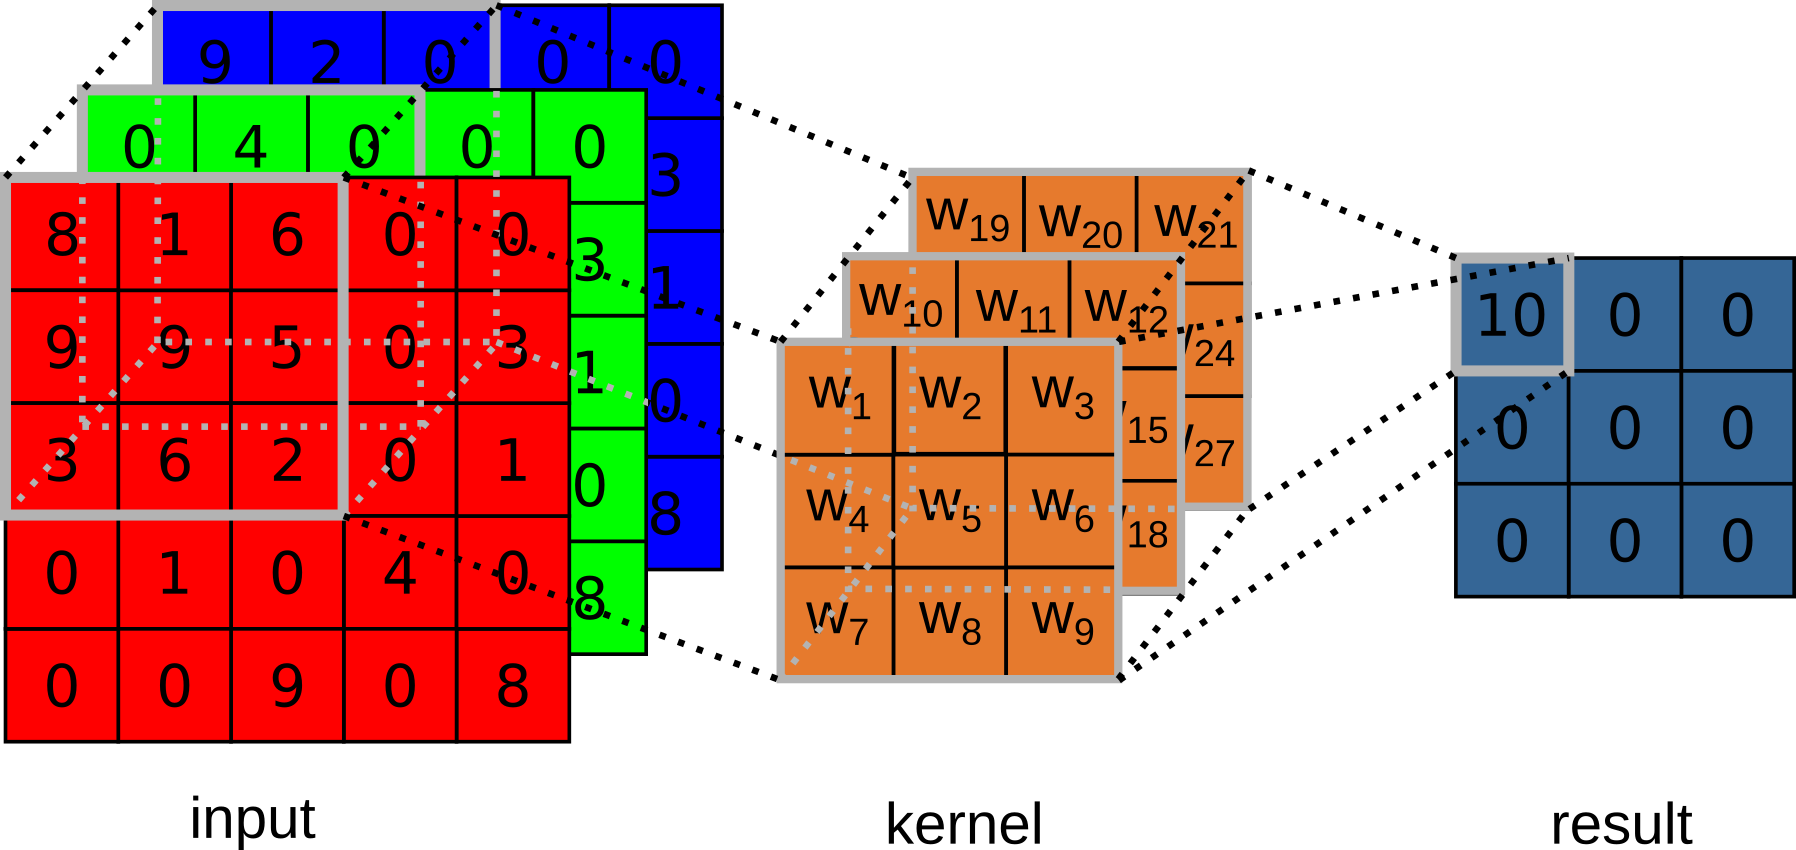
\includegraphics[scale=0.35]{images/figure118.png}
    \caption{Convolution of a 5x5x3 sized image with a 3x3x3 sized kernel and its result.}
    \label{fig:figure118}
\end{figure}

In Figure \ref{fig:figure119}, we have a representation of a convolution layer with more than one filter. For each one, we have an output and, consequently, we have in the final result a dataset where the number of depth layers (also known as feature map, illustrated by the three matrices in orange) will correspond to the number of filters applied to the input. This output can then be sent forward on the network, going through more convolutions and having more features extracted.

\begin{figure}
    \centering
    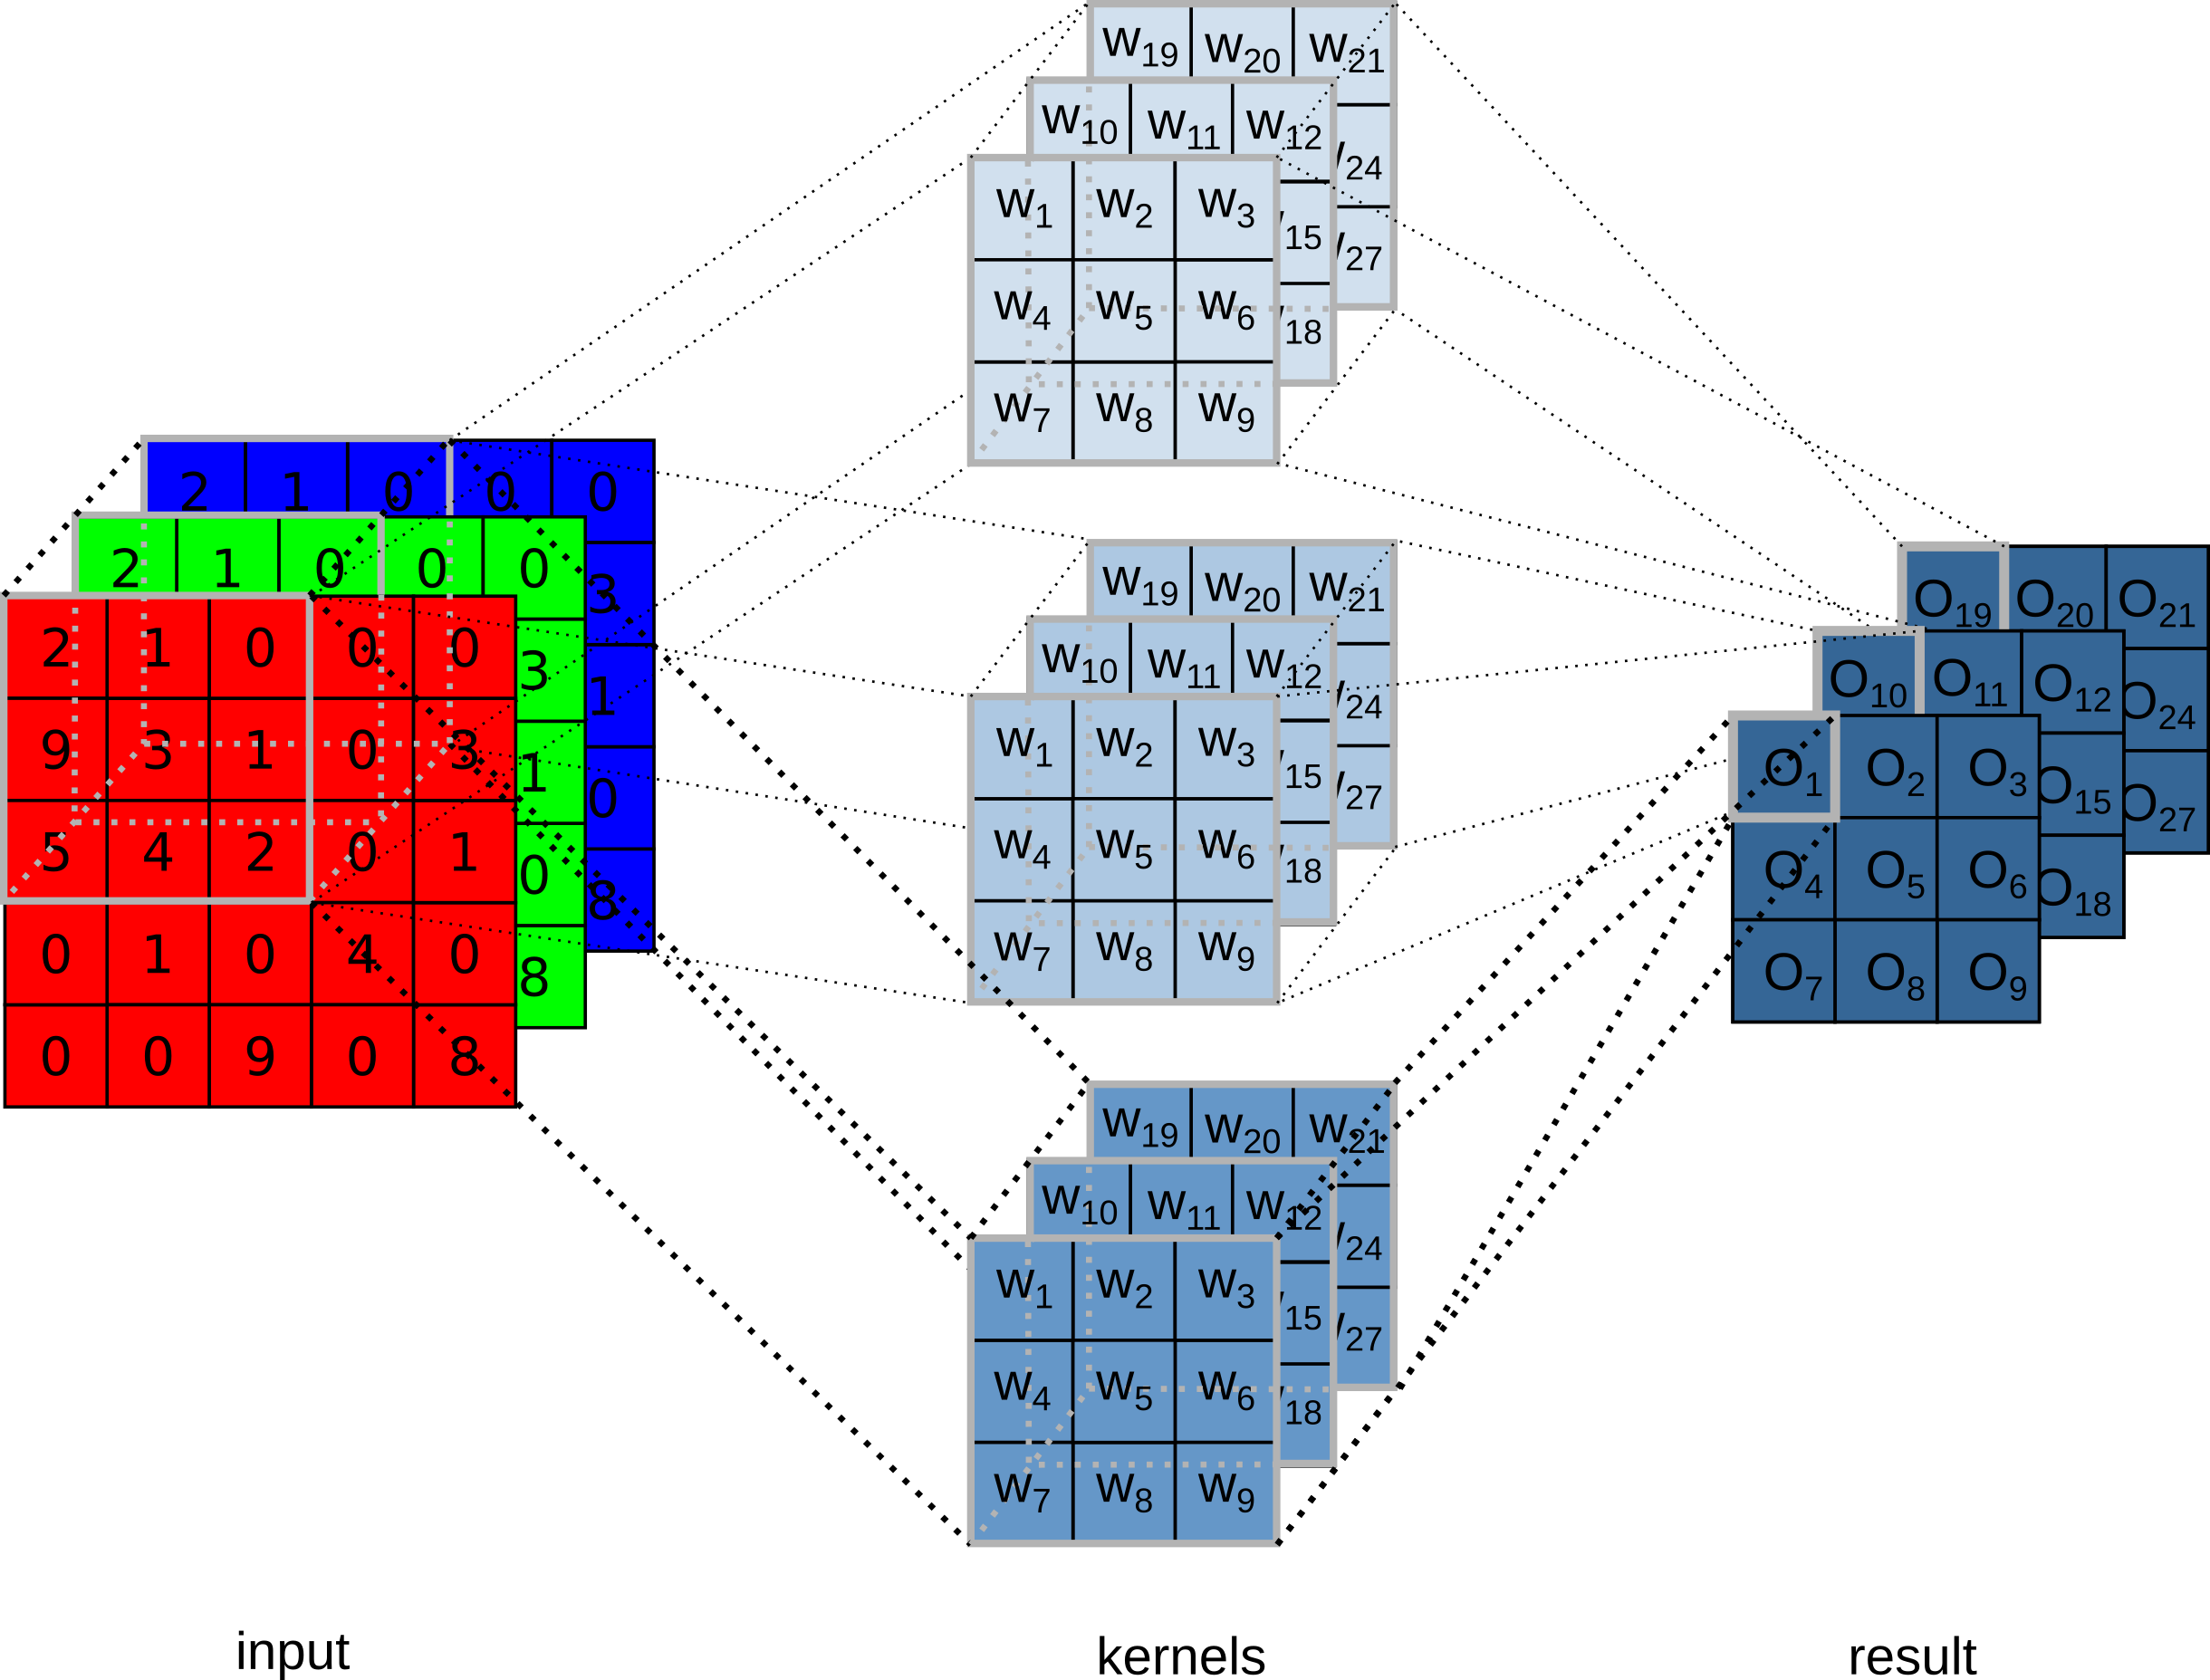
\includegraphics[scale=0.25]{images/figure119.png}
    \caption{Convolution of a 5x5x3 sized image with a 3x3x3 sized kernel and its result.}
    \label{fig:figure119}
\end{figure}

The two previous examples, Figures \ref{fig:figure117} and \ref{fig:figure119}, also serve to show us one of the features of convolution that make it a good choice for working with images, we call this feature sparse iterations (also known as sparse connectivity) \cite{goodfellow2016}. This attribute highlights the fact that each output unit, or pixel, is connected to only a fraction of the input units. In our previous example, each output is connected to a region of the 243 input pixels, 9x9x3. This is very useful, as our image can have millions of pixels, and using smaller sized kernels, we will be able to detect small features such as edges, corners, etc \cite{goodfellow2016}. In the convolution layers, the values that the network must learn are the values present in the filters, so that way we will have fewer parameters to learn and store. In a simple neural network, as we saw in the topic MLP network, an image at the input means that each pixel would be connected to each neuron in the next layer, thus resulting in an excessively large network.

Another important feature is the sharing of parameters, since the same filter is applied to different regions of the image using the same values, unlike a neural network without convolution layers, where we have a matrix with weights that are used for only one connection. The sharing of parameters gives us another feature, which is the invariance to translation, that is to say that if we move the position of an object in the input image, its representation will also be moved in the resulting image \cite{goodfellow2016}.

\subsection{Padding}

In the convolution examples, Figures \ref{fig:figure117} and \ref{fig:figure119}, we see that as we apply the kernel to the input image, the size of the output image is reduced. In fact, by convoluting a image of size $m x n$ with a filter of size $k_m x k_n$ the resulting image will have a height of $m-k_m+1$ and a length of $n-k_n+1$ . This type of convolution, where the resulting image is smaller, is often called “valid”.
If we want the output image to be the same size as the input image, we have to add more rows and columns to our image, this is known as padding. In this case, we use the formula  $m+2p-k_m+1$ and $n+2p-k_n+1$ where the padding represents. For example, in the previous Figures \ref{fig:figure117} and \ref{fig:figure119}, if we want an output equal in size to the input, we would have to use a padding of $6+2p-3+1=6p=1$.

\subsection{Stride}

The convolution examples we saw earlier used one-by-one displacement steps. But we can also use larger steps, as this reduces the computational cost of performing these steps at intervals. This clearly has an impact on the final result, decreasing its resolution, but in cases where we do not need to extract delicate features this becomes a good option \cite{goodfellow2016}.

When we use a stride value greater than one, this will also affect the output size, which will be governed by the following relationship \cite{adrian2017}:

\begin{equation}
\frac{m+2p-k_m}{s}+1 \  \times \ \frac{n+2p-k_n}{s}+1
\end{equation}

Where $m$ and $n$ are the image dimensions, p is the padding, $k_m$ and $k_n$ are the kernel dimensions and $s$ is the stride. In Figure \ref{fig:stride} we have an example with the steps of a convolution with stride=2 using a kernel of size 3 over an image of size 5 x 5 and padding=0.

\begin{figure}
    \centering
    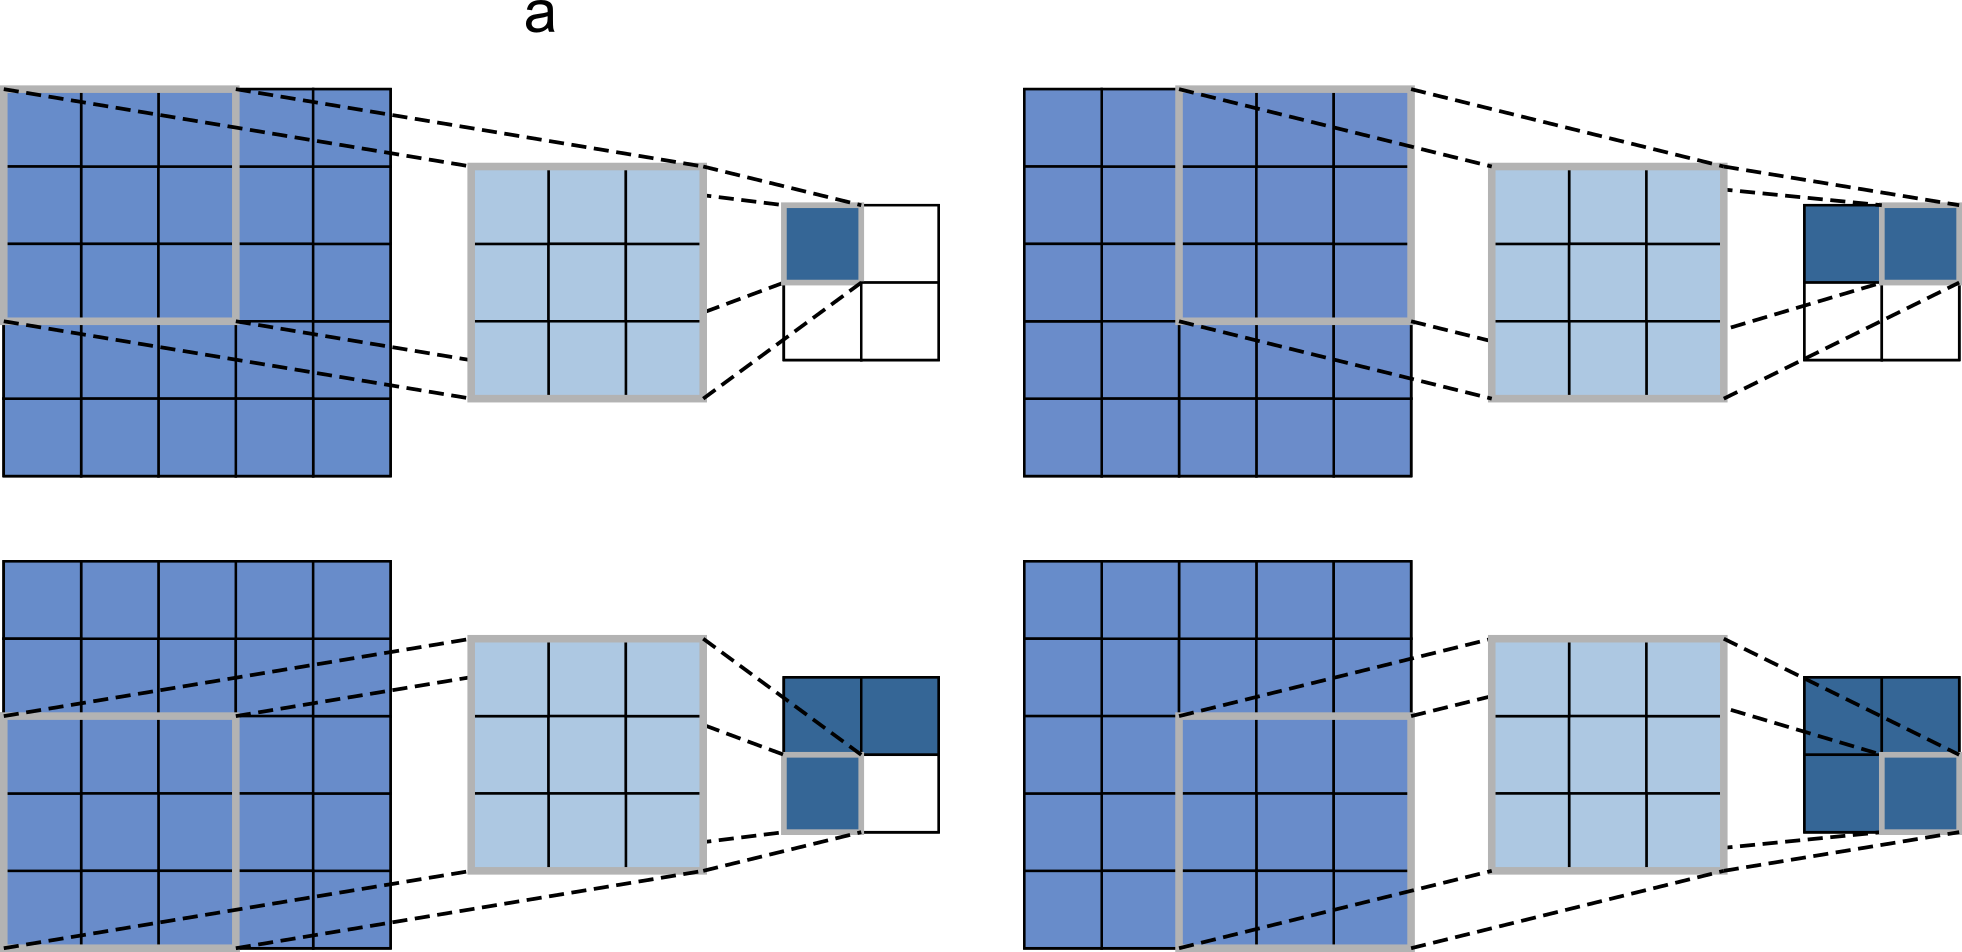
\includegraphics[scale=0.20]{images/stride.png}
    \caption{Example using stride bigger than 1.}
    \label{fig:stride}
\end{figure}

\subsection{Pooling}

This is a very important layer, which aims to subsampling the image to reduce its size, and, consequently, reduce the total memory, processing and parameters needed, in addition to curbing the risk of overfitting \cite{geron2019}\cite{adrian2017}\cite{elgendy2020}.

As in convolution layers each output unit is connected to an input region, so we must also take into account size, stride and padding. But, unlike convolution, the “kernel,” or, in other words, the region that will connect us to the input, will have no weights but only perform one operation, the most common being the maximum or the average \cite{geron2019} .

In Figure \ref{fig:figure121}, we have an example of max pooling, where we can see how it works in steps (Figures \ref{fig:figure121}(a-d)). This example uses a region of 2 x 2 , which is very common \cite{adrian2017}, and stride=1.

\begin{figure}
    \centering
    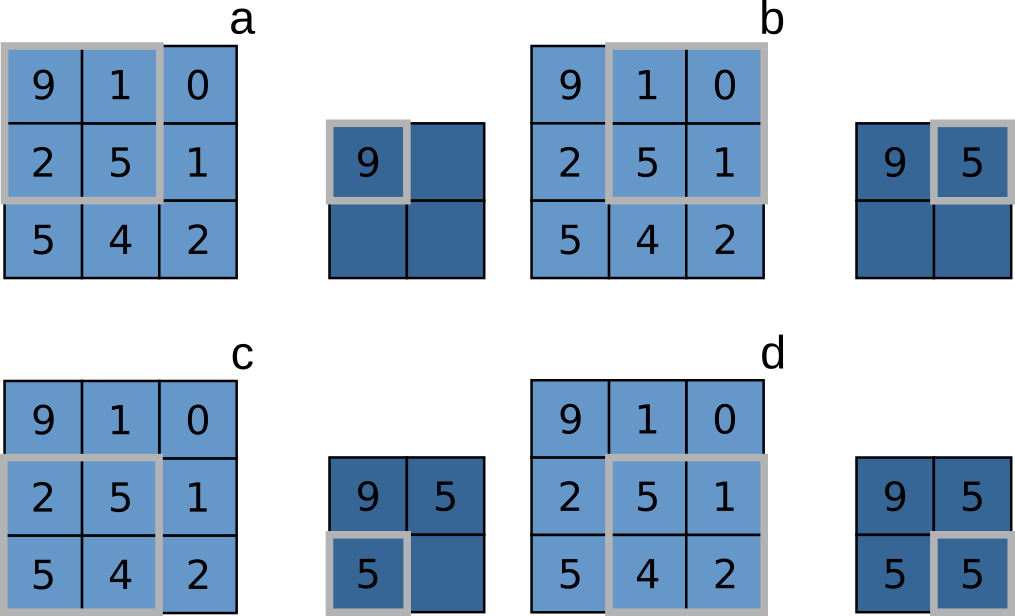
\includegraphics[scale=0.30]{images/figure121.png}
    \caption{Example of max pooling application.}
    \label{fig:figure121}
\end{figure}

In Figure \ref{fig:figure122}, we have another example of max pooling, but this time performed with a larger input, we can see that the operation is performed on each input layer of the object, and that its output contains the same number of layers as the input, which is what typically occurs in this type of operation \cite{geron2019}.

\begin{figure}
    \centering
    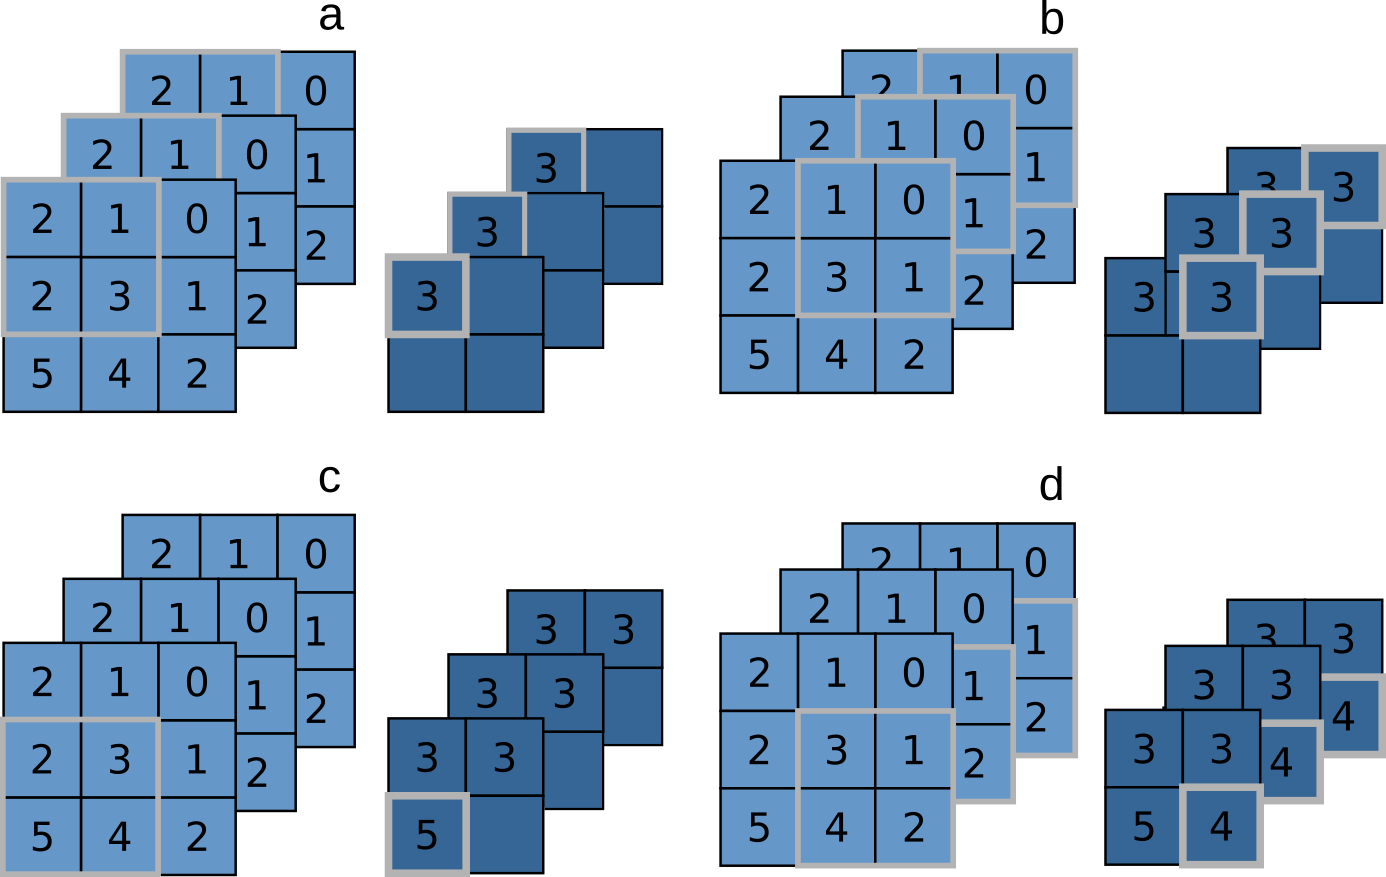
\includegraphics[scale=0.30]{images/figure122.png}
    \caption{Example of max pooling application in an image with more dimensions.}
    \label{fig:figure122}
\end{figure}

Although pooling is a very widespread technique, we can find networks where their authors preferred not to use pooling to perform subsampling, but to use convolution layers with higher stride and padding values to achieve this dimension reduction \cite{elgendy2020}\cite{adrian2017}. This way of working was proposed by Springenberg et al. in their 2014 article “Striving for Simplicity: The All Convolutional Net”, where they demonstrate that even networks without pooling layers can have good results in different databases, such as CIFAR-10 and ImageNet.

\subsection{Fully Connected Layers}

CNN's usually have several convolution layers followed by activation functions, which in turn are followed by pooling layers, and this process decreases the dimensions m x n and increases the depth, that is, the number of feature layers (known as feature maps ) \cite{elgendy2020}\cite{geron2019}. In Figure \ref{fig:figure123}, we have a representation of this process through the network topology. At the end of this network we have a large amount of layers with the characteristics extracted from the input image, and we need to use this information. In this same Figure, we can see that in the end we have fully connected layers, which is a regular neural network, an MLP \cite{elgendy2020}.

\begin{figure}
    \centering
    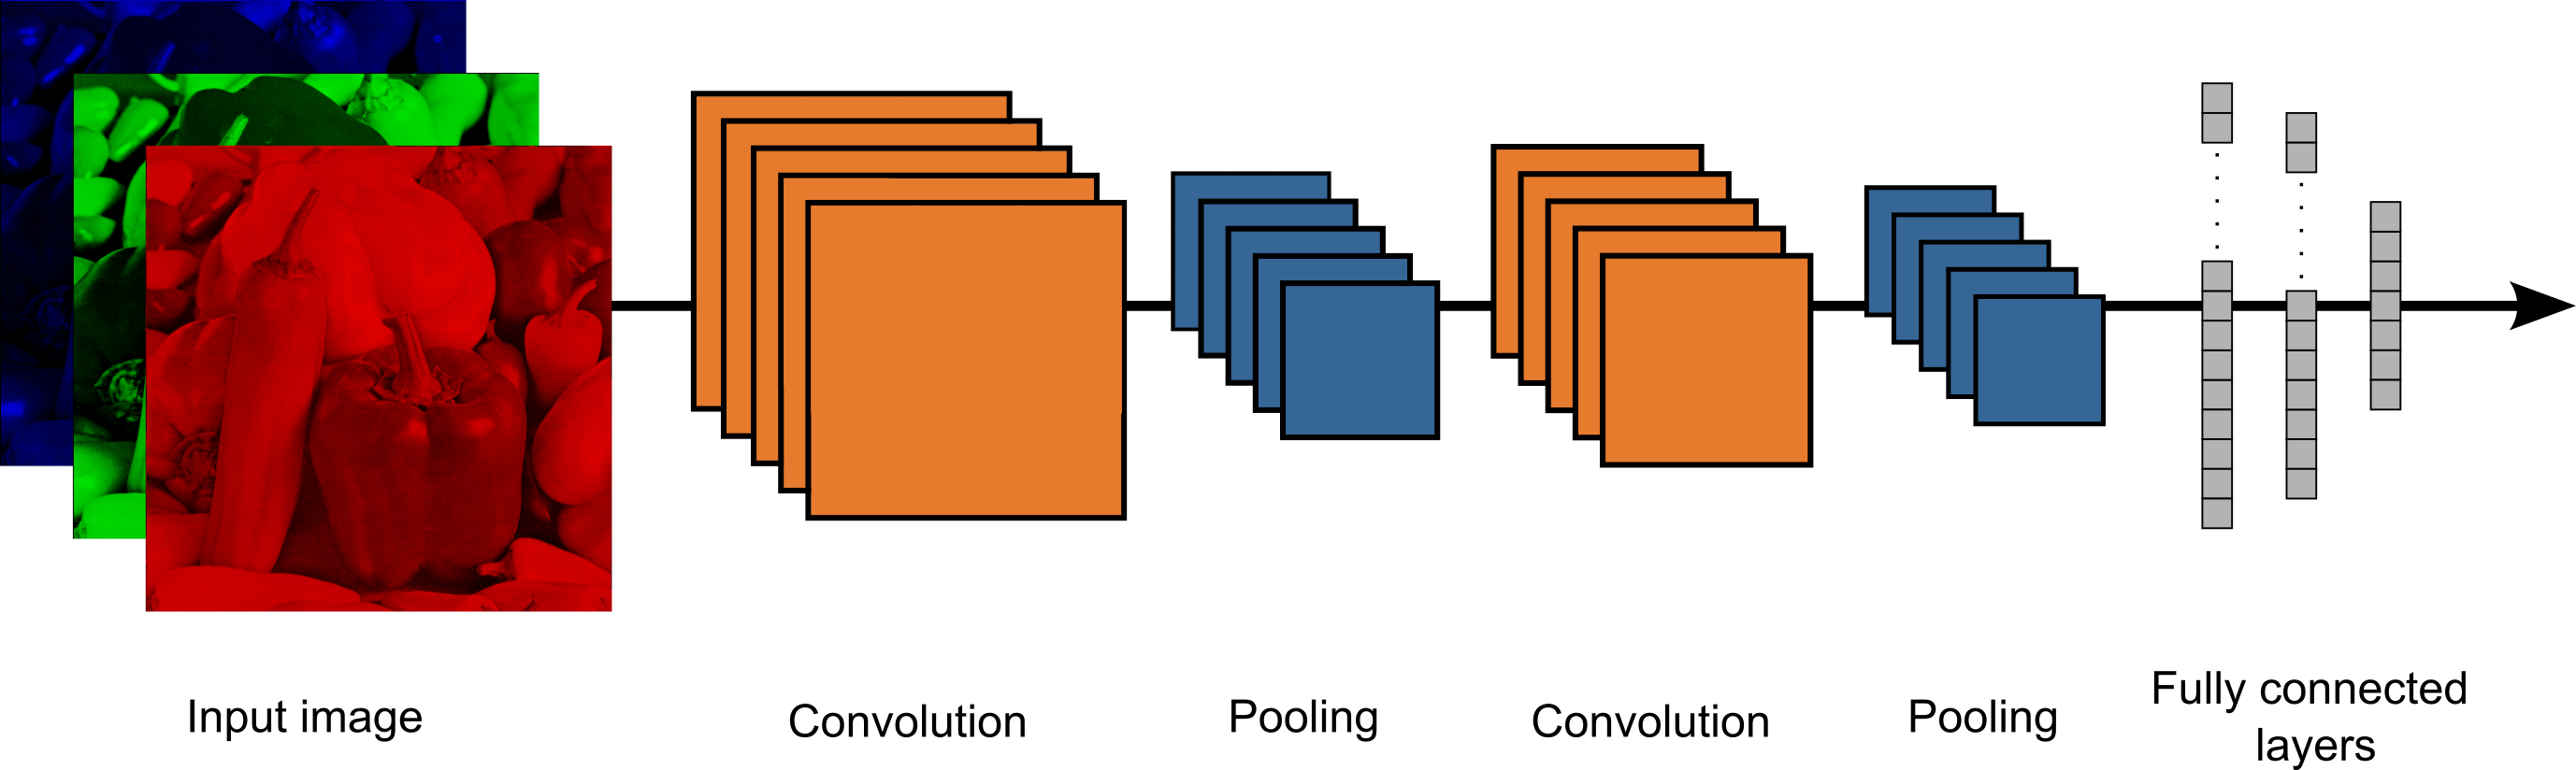
\includegraphics[scale=0.22]{images/figure123.png}
    \caption{Example of max pooling application in an image with more dimensions.}
    \label{fig:figure123}
\end{figure}

In Figure \ref{fig:figure124} we have the representation of the use of the information abstracted from the image by the convolution layers. In this exemple, the data ends with a size of 7x7x64, that is, we have 64 feature maps with a size of 7x7. To provide this data to the full connected layer, we have to flatten these feature maps to a vector of dimensions 1x3136, that passes through the network and ends in the layer of Softmax, that produces the output vector.

\begin{figure}
    \centering
    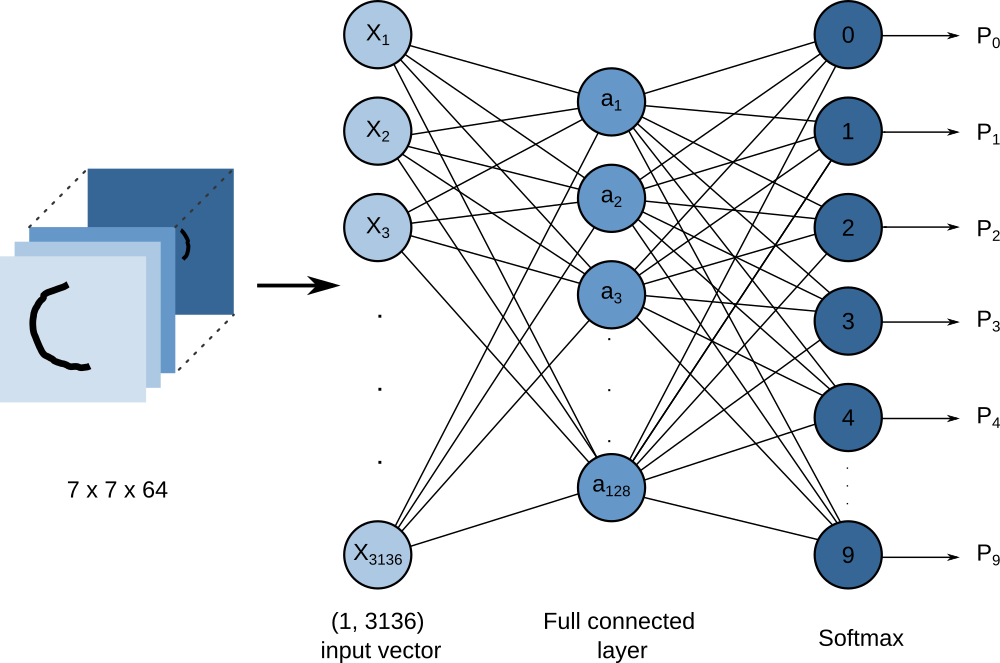
\includegraphics[scale=0.50]{images/figure124.png}
    \caption{Example of max pooling application in an image with more dimensions.}
    \label{fig:figure124}
\end{figure}

